\documentclass{article}
\usepackage{MnSymbol,utfsym,arev}
\usepackage{wrapfig}
\usepackage{placeins}
\usepackage{graphicx} % Required for inserting images
%AT Lab Final Report Format
\title{\textbf{AgriConnect: A Farmer Marketplace}}
\author{Harshita Gupta (210911224)\\
        Aastha Sinha (210911320)\\
        Charu Yadav (210911396)}
\date{March 2024}

\begin{document}

\maketitle
\textbf{Abstract:}
This innovative app bridges the gap between small farmers and merchants, streamlining the agricultural supply chain through direct and efficient market access. Utilizing phone number-based authentication for inclusivity, it facilitates the listing and purchasing of crops, enhancing transactional transparency and trust. The app supports essential features such as listing management, real-time status updates, and secure transaction recording, tailored for users with limited access to digital banking services. Designed to empower the grassroots of the agricultural sector, it fosters economic growth and sustainability. Available in English and Hindi, it addresses the linguistic diversity of its user base, making technology accessible and beneficial for small-scale agriculture.\\

\textbf{KEYWORDS: Small Farmers, Merchants, Marketplace App, Sustainable Agriculture, Local Economy}

\section{Introduction}
\label{sec:introduction}

In an endeavor to revolutionize the agricultural marketplace, our project introduces a mobile application specifically designed to empower small farmers and merchants by facilitating direct trade and mitigating the logistical and economic disadvantages currently faced. The scope of our work extends to dismantling the barriers imposed by traditional supply chains, leveraging advanced technologies to provide a seamless and accessible platform. The prevalent issues within the agricultural sector—restricted market access, reliance on intermediaries that dilute profits, and a significant digital divide—underscore the urgency and necessity of our solution. A substantial majority of small-scale agriculturalists are sidelined from the digital economy due to the lack of simple, accessible digital tools, particularly those without standard email access for authentication purposes.\\

Our application addresses these challenges head-on by implementing phone number-based authentication via Firebase, negating the need for email IDs and thus broadening accessibility. It enables farmers to list their crops for sale and merchants to easily discover and purchase these goods, all within a user-friendly interface that supports real-time updates and direct communication facilitated by Dialogflow. The app not only accommodates offline payments to include users with limited digital payment access but also offers multi-lingual support, ensuring inclusivity across diverse linguistic backgrounds. The decision to employ Firestore as our database solution reflects our commitment to scalability and flexibility, essential for adapting to the evolving needs of our user base.\\

By directly connecting farmers and merchants, our application aims to streamline transactions, enhance market transparency, and promote sustainable agricultural practices. Through this initiative, we aspire to foster a more equitable and efficient marketplace, where small farmers and merchants can thrive, free from the constraints of traditional intermediaries, and where consumers can benefit from a more diverse and accessible supply of agricultural products.\\

Our contribution lies in developing an innovative mobile app designed to empower small farmers and merchants by facilitating direct agricultural trade. Leveraging phone number-based login via Firebase for broad accessibility, our app simplifies the buying and selling process, enabling farmers to list crops and merchants to easily purchase them. It features a straightforward UI, real-time listing updates, secure transaction recording, and a bilingual interface in English and Hindi to cater to a diverse user base. By integrating Dialogflow for efficient communication and Firestore for robust data management, we're addressing the digital divide, enhancing market transparency, and supporting the economic growth of small-scale agriculturalists.\\

\section{Literature Review}

M. Bhende et al., [1] introduces a digital market platform tailored for farmers, facilitating e-commerce activities to streamline agricultural transactions. It aims to empower farmers by leveraging technology to enhance market access and efficiency in the agricultural sector.\\

S. Rahayu., [2] presents an e-commerce platform utilizing the marketplace model to facilitate the sale of agricultural products. It adopts the Xtreme programming approach to enhance the development process and ensure a robust, customer-centric solution for agricultural market transactions.\\

Imesha et al., [3] outlines the development of a conceptual mobile application prototype aimed at connecting Sri Lankan farmers with retailers digitally. It focuses on bridging the gap between agricultural producers and buyers, potentially transforming the agricultural supply chain through technological innovation.\\
    
R. Deshmukh et al., [4] explores the implementation of e-business solutions in agriculture to facilitate communication between merchants and farmers. It highlights the importance of leveraging digital platforms to enhance efficiency and effectiveness in agricultural transactions and interactions.\\

    A. Raj et al., [5] details the development of a mobile application specifically designed to provide agro-advisory services to farmers, focusing on their needs and preferences. It aims to empower farmers with timely and personalized advice, leveraging mobile technology to enhance agricultural productivity and decision-making.\\
    
    A. Singh et al., [6] presents a comprehensive review of mobile applications tailored for farmer-centric agriculture, highlighting their features and functionalities. It aims to provide insights into the existing landscape of agricultural mobile apps, assessing their potential impact on enhancing farmer productivity and welfare.\\
    
    S. Ahmad et al., [7] offers a thorough review of mobile applications designed for farmers, examining their current status and future prospects. It aims to provide valuable insights into the landscape of agricultural mobile apps, identifying potential areas for improvement and future development directions.\\
    
    Y. Zhai et al.,[8] conducts a survey focusing on mobile agricultural applications from a user perspective, aiming to understand user preferences and challenges. It provides insights into the usability and effectiveness of existing mobile apps in meeting the needs of agricultural stakeholders, informing future development efforts.\\
    
    A. P. Muhammed et al.,[9] introduces "AGRIO APP," an advanced Android application tailored specifically for farmers. It aims to provide comprehensive features and functionalities to support various agricultural activities, enhancing productivity and decision-making among farmers.\\
    
    K. Gurjar et al., [10] presents the development of a mobile application aimed at connecting farmers with traders, alongside a price prediction model utilizing machine learning techniques. It addresses the need for improved market access and pricing information for farmers, leveraging technology to enhance their decision-making capabilities and market interactions.\\
    
    A. Bhandari et al., [11] presents an Android application designed to empower farmers to sell their produce at better rates. It addresses the challenges faced by farmers in accessing fair market prices, providing a platform for improved market participation and profitability.\\
    
    M. Dane et al., [12] introduces "E-Farming Bazaar," a platform designed to facilitate agricultural transactions and market interactions. It aims to harness digital technology to streamline farming activities and improve market access for farmers, potentially transforming the agricultural landscape.
\end{enumerate}

\subsection{Research Gap}
\begin{enumerate}
  \item Limited emphasis on supporting multi-farmer purchases is a common research gap.[5][6][9][10][11]
  \item Real-time updates on crop availability are lacking.[2][5][7][12]
  \item Explicit mention of chat support in various regional languages is notably absent, hindering accessibility for diverse users. [1][3][6][8]
\end{enumerate}

\subsection{Objectives}
Farmer-Centric Agriculture Marketplace aims to provide a comprehensive and efficient platform that connects farmers with buyers, streamlines agricultural transactions, and supports the growth of a thriving agricultural community. This system focuses on enhancing the user experience for farmers and merchants while ensuring 
\begin{enumerate}
    \item Implements secure, phone-based OTP authentication to enhance accessibility and user trust.
    \item Features a user-friendly homepage for easy navigation of app functionalities, optimizing user experience.
    \item Provides real-time tracking of crop listings for farmers, including status updates and merchant interactions, to ensure transaction transparency.
    \item Facilitates a dynamic marketplace where users can explore and engage with a wide range of listings, fostering trade opportunities.
    \item Simplifies the transaction process with support for both offline and digital payments, streamlining user transactions.
    \item Integrates chat functionality for immediate user support, aiming to reduce issues and enhance satisfaction.
    \item Offers a clear logout feature to safeguard user privacy and reinforce security measures.
\end{enumerate}

\subsection{Contribution/Novelty}
\begin{enumerate}
    \item \textbf{Promotion of Agricultural Sustainability (SDG 2):} By providing a platform for small farmers to directly access markets and fair prices for their produce, our app helps reduce food waste and increase the profitability of farming, contributing to sustainable agriculture.
    
    \item \textbf{Fostering Partnerships (SDG 17):} The app acts as a bridge between various stakeholders in the agricultural sector, including farmers, merchants, technology providers, and financial institutions. By leveraging technology to create a community of practice, it fosters partnerships that are crucial for sharing knowledge, resources, and best practices, thereby strengthening the means of implementation and revitalizing the global partnership for sustainable development.
    
    \item \textbf{Encouragement of Responsible Consumption and Production (SDG 12):} By facilitating direct transactions between producers and consumers, the app encourages the consumption of local produce, reducing the carbon footprint associated with long supply chains. It also supports small-scale producers in adopting sustainable practices by providing them with a platform to market their sustainably grown produce directly to conscious consumers.
    
    \item \textbf{Support for Economic Growth and Decent Work (SDG 8):} The app empowers small farmers and merchants by offering them greater control over their sales and purchases, leading to increased incomes, sustained economic growth, and decent job creation within rural communities. By bypassing traditional intermediaries, farmers receive a fairer share of profits, promoting inclusive and sustainable economic growth.
\end{enumerate}

Our app is not just a marketplace but a tool for social and economic change, designed to make the agricultural supply chain more transparent, equitable, and sustainable. By leveraging technology to empower small farmers and merchants, the app directly contributes to the achievement of the SDGs, making it a distinctive and efficient solution in the global effort to promote sustainability.

\begin{table}[htbp]
  \centering
  \begin{tabular}{|p{1cm}|p{1.2cm}|p{1.2cm}|p{1.2cm}|p{1.2cm}|p{1.2cm}|p{1.2cm}|p{1.2cm}|p{1.2cm}|p{1.5cm}|}
      \hline
      \textbf{Paper} & \textbf{Auth} & \textbf{Crop Listing} & \textbf{Merchant Listing} & \textbf{Multi Farmer Purchase} & \textbf{Chat-Bot} & \textbf{Add Listing} & \textbf{Real-Time Crop Updates} & \textbf{Regional Language support}\\
      \hline
      [1] & N & Y & N & Y & Y & N & N & Y \\
      \hline
      [2] & Y & Y & Y & Y & Y & Y & N & N \\
      \hline
      [3] & Y & Y & Y & Y & N & N & N & Y \\
      \hline
      [4] & Y & Y & N & Y & Y & N & N & N \\
      \hline
      [5] & Y & Y & N & N & N & N & Y & N \\
      \hline
      [6] & Y & N & N & N & N & N & N & N \\
      \hline
      [7] & Y & Y & Y & Y & Y & Y & N & Y \\
      \hline
      [8] & Y & Y & Y & N & N & Y & N & N \\
      \hline
      [9] & Y & Y & N & N & N & N & Y & Y \\
      \hline
      [10] & Y & Y & N & N & N & N & N & Y \\
      \hline
      [11] & Y & Y & N & N & N & Y & Y & N \\
      \hline
      [12] & Y & Y & N & N & N & N & N & Y \\
      \hline
      Our App & Y & Y & Y & Y & Y & Y & Y & Y \\
      \hline
  \end{tabular}
  \caption{Comparison with other literary papers}
  \label{tab:comparison}
\end{table}
\FloatBarrier
\section{Methodology}
The methodology for developing AgroConnect, our innovative app designed to empower small farmers and merchants, adopts a comprehensive approach that intertwines technical development with user-centric design principles. Initially, the project embarked on an extensive requirement gathering phase, employing user stories and stakeholder interviews to meticulously outline the app's primary functionalities such as user registration via OTP, real-time listing and transaction management, and direct communication channels. This foundational step ensured that the app's design and features aligned closely with the actual needs and preferences of its target audience. Following the requirement analysis, the project leveraged agile development methodologies, facilitating rapid prototyping, iterative testing, and continuous feedback integration to enhance app usability and performance. The technical architecture was meticulously planned, choosing Kotlin for its modern syntax and compatibility with Android Jetpack components to ensure robust and scalable app development. Firestore was selected for the database to capitalize on its real-time data synchronization capabilities, essential for the dynamic listing and transaction features envisioned. Firebase Authentication was integrated to streamline user access with secure OTP verification, catering to the app's diverse user base with varying levels of digital access. Throughout the development process, special emphasis was placed on creating an intuitive user interface, with XML layouts designed for simplicity and ease of navigation, ensuring the app remains accessible to users with limited technological proficiency. Security and privacy were paramount, with data encryption and secure communication channels implemented to protect user information. The app also underwent rigorous testing phases, including performance optimization and user acceptance testing, to refine functionality and ensure reliability. By adopting a user-centered development approach, AgroConnect was crafted not just as a marketplace app but as a tool for economic empowerment and sustainability in the agricultural sector, aiming to bridge the gap between small-scale producers and the market effectively. The architecture of This app is being shown in Figure 1.
\begin{figure}[htbp]
  \centering
  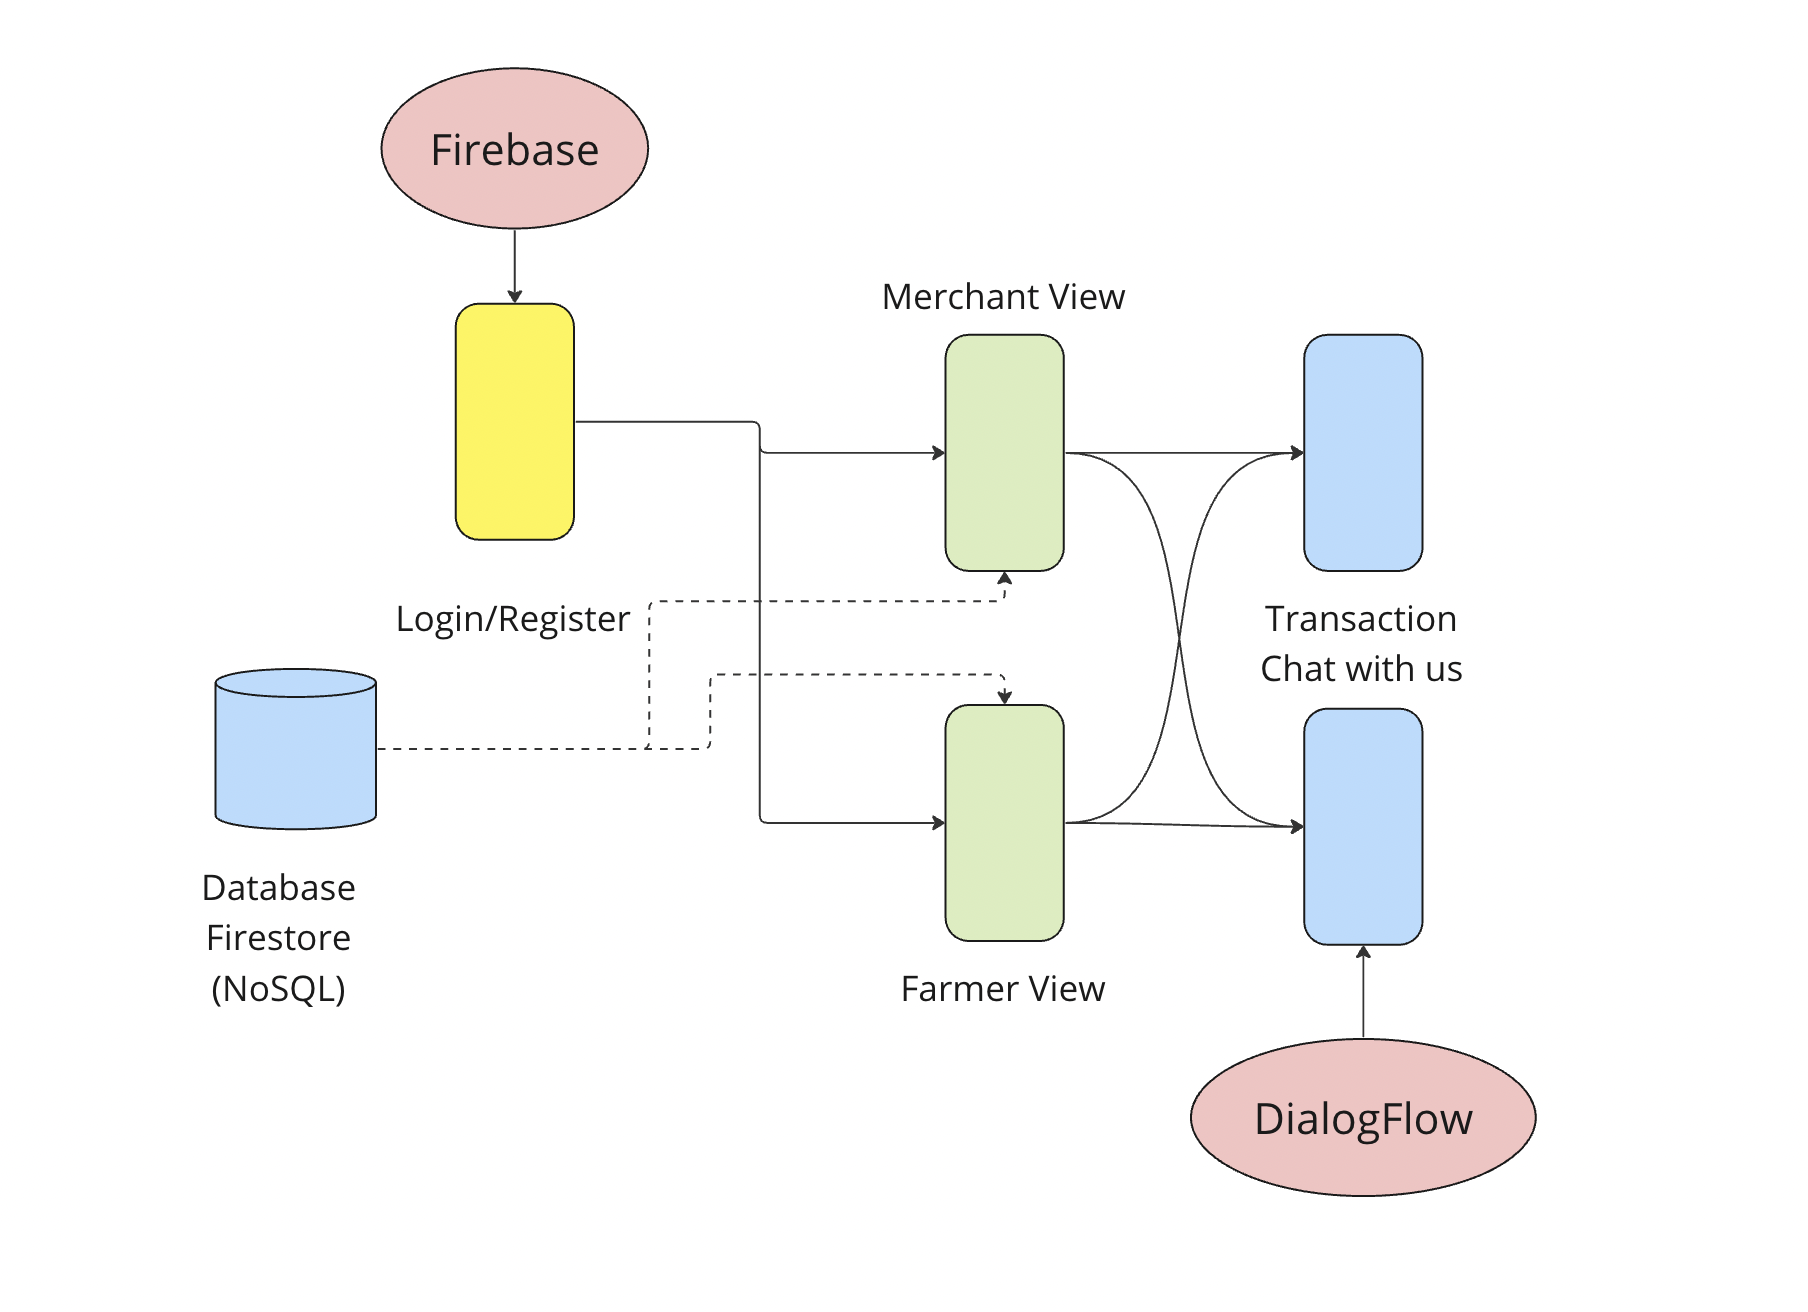
\includegraphics[width=01\linewidth]{arch.png}
  \caption{Architecture Diagram}
\end{figure}
\FloatBarrier
\subsection{LLD}
\begin{enumerate}
    \item \textbf{Languages and Framework:}
    \begin{itemize}
        \item Utilizes Kotlin for streamlined backend logic and leverages the Android Jetpack components for modern, robust application development.
        \item Employs XML for crafting intuitive and responsive layouts for various screens and user interface components.
    \end{itemize}
    
    \item \textbf{Database Schema:}
    \begin{itemize}
        \item Adopts Firestore, a flexible, scalable NoSQL cloud database, to store user profiles, crop listings, transactions, and chat messages.
        \item Structures collections for users, listings (with sub-collections for farmer listings and merchant listings), transactions, and chats.
    \end{itemize}
    
    \item \textbf{User Authentication and Authorization:}
    \begin{itemize}
        \item Integrates Firebase Authentication to provide a secure and hassle-free sign-in experience using phone numbers and OTP.
        \item Establishes user roles (farmer or merchant) upon signup to tailor app functionality and permissions appropriately.
    \end{itemize}
    
    \item \textbf{Marketplace Functionality:}
    \begin{itemize}
        \item Implements Firestore queries to enable real-time listing of crops, viewing of listings, and updates on transaction statuses.
        \item Develops mechanisms for adding, editing, and removing listings, with updates reflected in real-time across the platform.
    \end{itemize}
    
    \item \textbf{Transaction Process:}
    \begin{itemize}
        \item Designs a simple yet effective transaction process to record and track payments, accommodating users with limited access to digital payment methods.
        \item Ensures transparency and security in the transaction process, providing users with a record of all transactions completed through the app.
    \end{itemize}
    
    \item \textbf{Network Communication:}
    \begin{itemize}
        \item Utilizes Google Cloud Functions for server-side logic and integrating external APIs for SMS notifications and OTP verification.
        \item Employs robust error handling and network communication strategies to manage data transfer efficiently and securely.
    \end{itemize}
    
    \item \textbf{Security \& Privacy:}
    \begin{itemize}
        \item Enforces data encryption for sensitive information stored in Firestore and transmitted over the network to safeguard user privacy.
        \item Adheres to best practices in data storage and access, ensuring that user information is protected according to privacy laws and regulations.
    \end{itemize}
    
    \item \textbf{Performance Optimisation:}
    \begin{itemize}
        \item Applies caching strategies and Firestore data optimization to enhance app performance, particularly in rural areas with limited connectivity.
        \item Conducts thorough performance testing to identify and mitigate any potential bottlenecks, ensuring a smooth user experience.
    \end{itemize}
\end{enumerate}
We have shown the Activity Diagram for Low-Level Design in Figure 2.
\begin{figure}[]
  \centering
  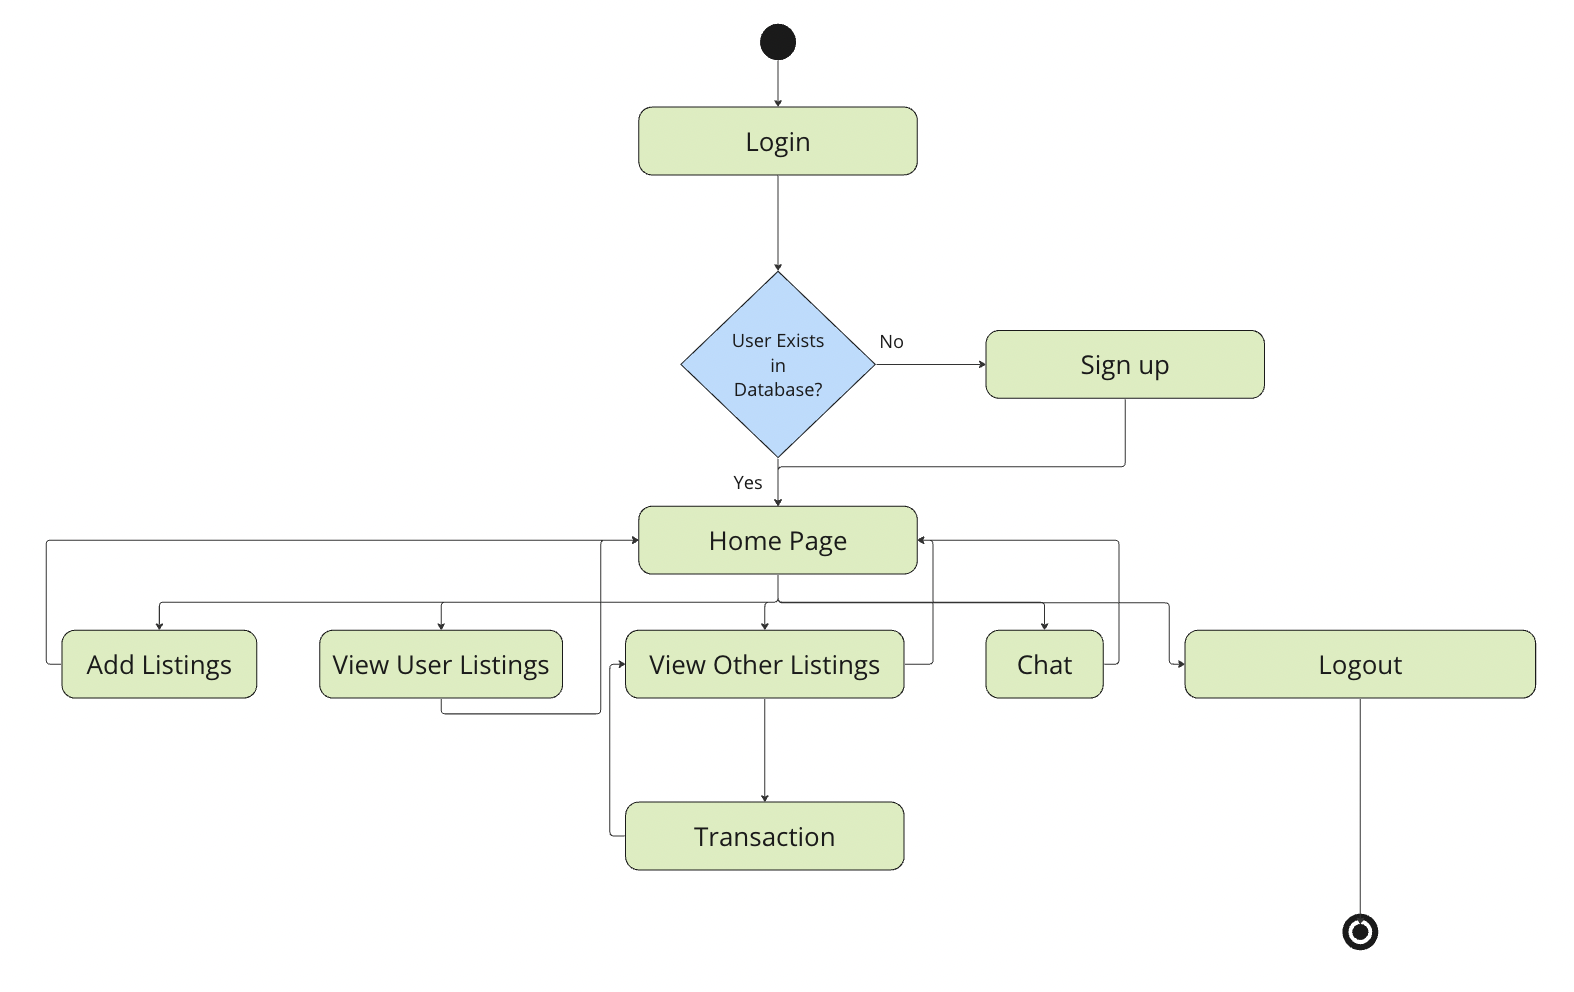
\includegraphics[width=1\linewidth]{image2.png}
  \caption{Activity Diagram}
\end{figure}
\FloatBarrier
\subsection{HLD}
\textbf{System Overview:}
AgriConnect is designed to facilitate direct trade between small farmers and merchants, streamlining the agricultural marketplace through technology.\\

\textbf{Modules:}
\begin{enumerate}
    \item \textbf{User Authentication Module:} Manages secure login and signup processes, utilizing phone number verification.
    \item \textbf{Listing Management Module:} Allows users to create, view, and manage crop listings, tailored to either the farmer or merchant role.
    \item \textbf{Transaction Module:} Handles the recording and viewing of transactions, providing a transparent history of purchases and sales.
    \item \textbf{Chat Module:} Enables direct communication between users for inquiries and negotiations related to listings.
    \item \textbf{User Role Management:} Distinguishes between farmers and merchants, customizing the app experience to suit each user's needs.
    \item \textbf{Profile and Settings Module:} Offers users the ability to manage their profile and app settings, including bank details for transactions.
\end{enumerate}

\textbf{Key Features Implementation:}

\begin{enumerate}
    \item \textbf{Direct Marketplace Access:} Employs an intuitive UI/UX design to facilitate the listing and purchasing process.
    \item \textbf{Role-Based Functionality:} Customizes the app experience for farmers and merchants, enhancing usability and relevance.
    \item \textbf{Simple Transactions:} Implements a straightforward process for recording transactions, ensuring trust and reliability.
    \item \textbf{Real-Time Listings Update:} Leverages Firestore for live updates to listings and transactions, keeping all users informed.
    \item \textbf{Multi-Lingual Support:} Offers the app in English and Hindi, broadening accessibility for users in diverse regions.
\end{enumerate}

\textbf{Enhanced User Experience:}

\begin{enumerate}
    \item \textbf{Efficient Navigation:} Utilizes Android's Navigation component for seamless movement between different sections of the app.
    \item \textbf{Responsive Design:} Ensures the app is accessible on various devices and screen sizes, providing a consistent user experience.
\end{enumerate}

\textbf{Data Flow:} 
User interactions are systematically directed through the app's modules, ensuring a coherent flow from authentication to transactions.\\

\textbf{Technology Stack:}

\begin{enumerate}
    \item \textbf{Kotlin and Android Jetpack} for the Android app development.
    \item \textbf{Firebase Authentication} for secure login mechanisms.
    \item \textbf{Firestore} for real-time database needs.
    \item \textbf{Google Cloud Functions} for server-side logic.
\end{enumerate}
We have shown the Sequence Diagram for High-Level Design in Figure 3.
\begin{figure}[htbp]
  \centering
  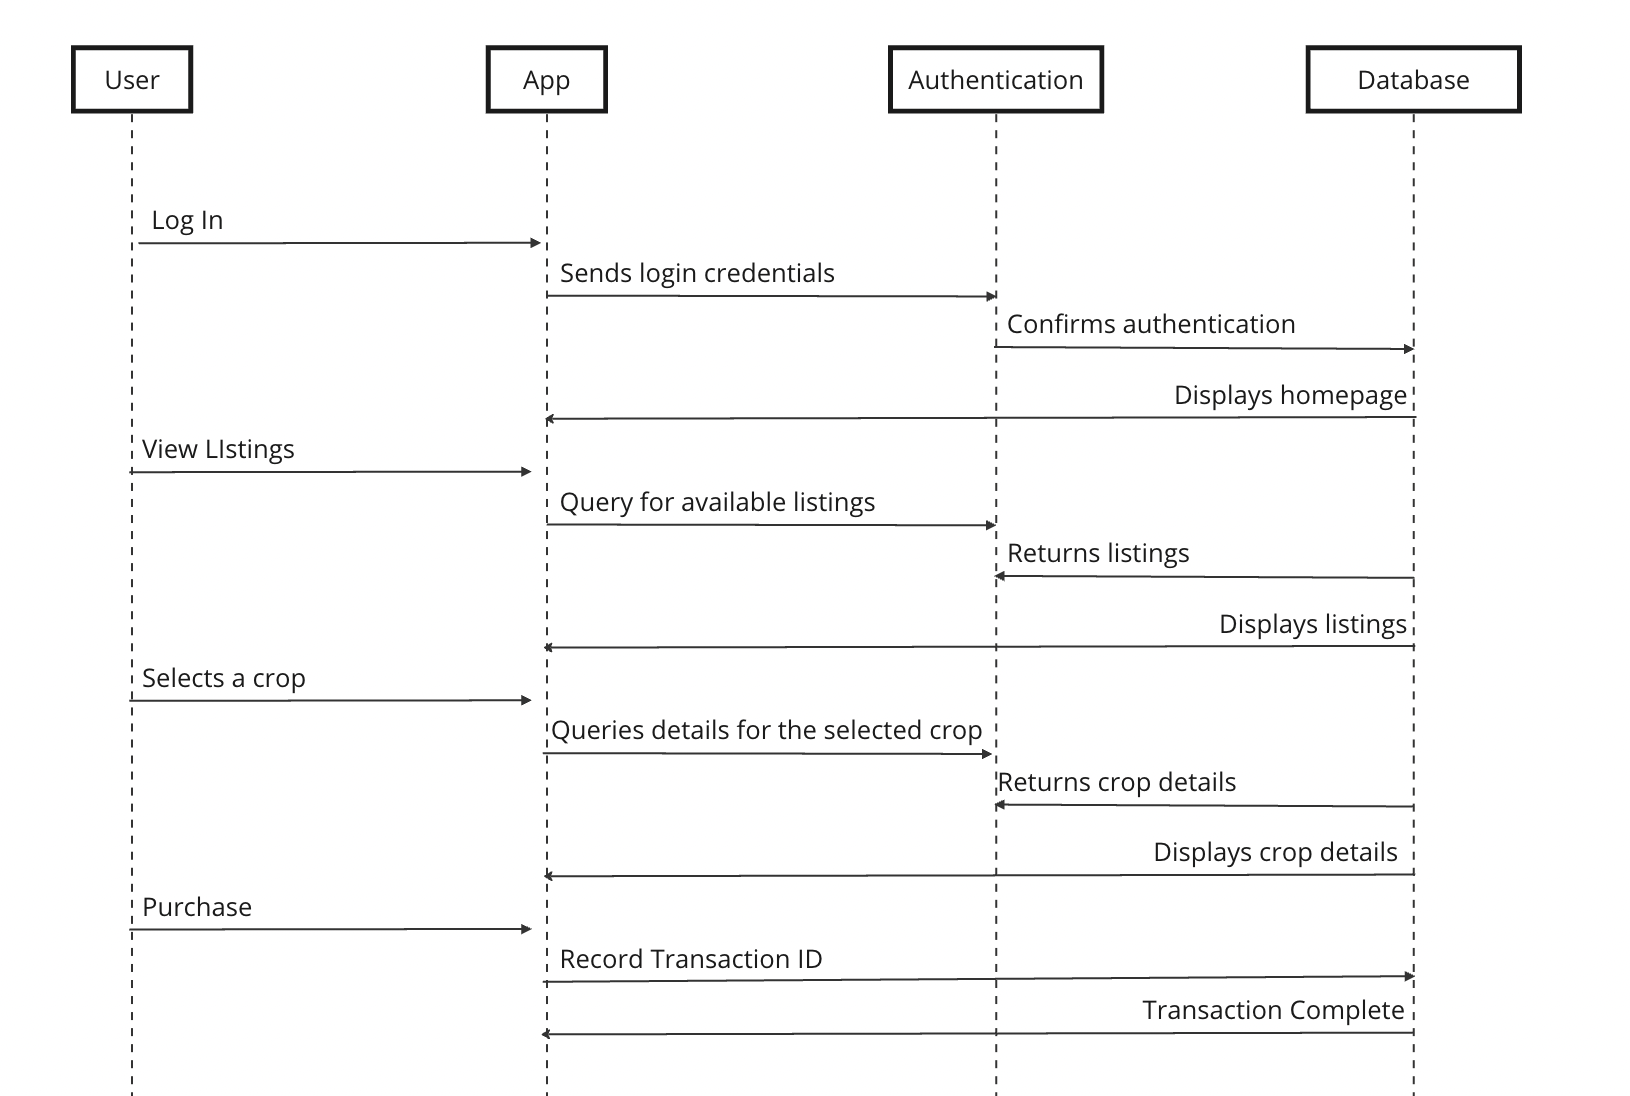
\includegraphics[width=1\linewidth]{image.png}
  \caption{Sequence Diagram}
\end{figure}
\FloatBarrier

\section{Results}
Figure 4 shows a login page where the user can log on to his account. Figure 5 shows the authentication page where we verify using OTP. Figure 6 shows the Home page where we enter after verification. Figures 7, 8, 9 and 10 show listing for users.  Figure 10 also shows an Accept button to make transactions further. The transaction page is shown in Figure 12. Figure 11 shows the page to add listings for both users.\\
\begin{figure}[htbp]
  \centering
  \fbox{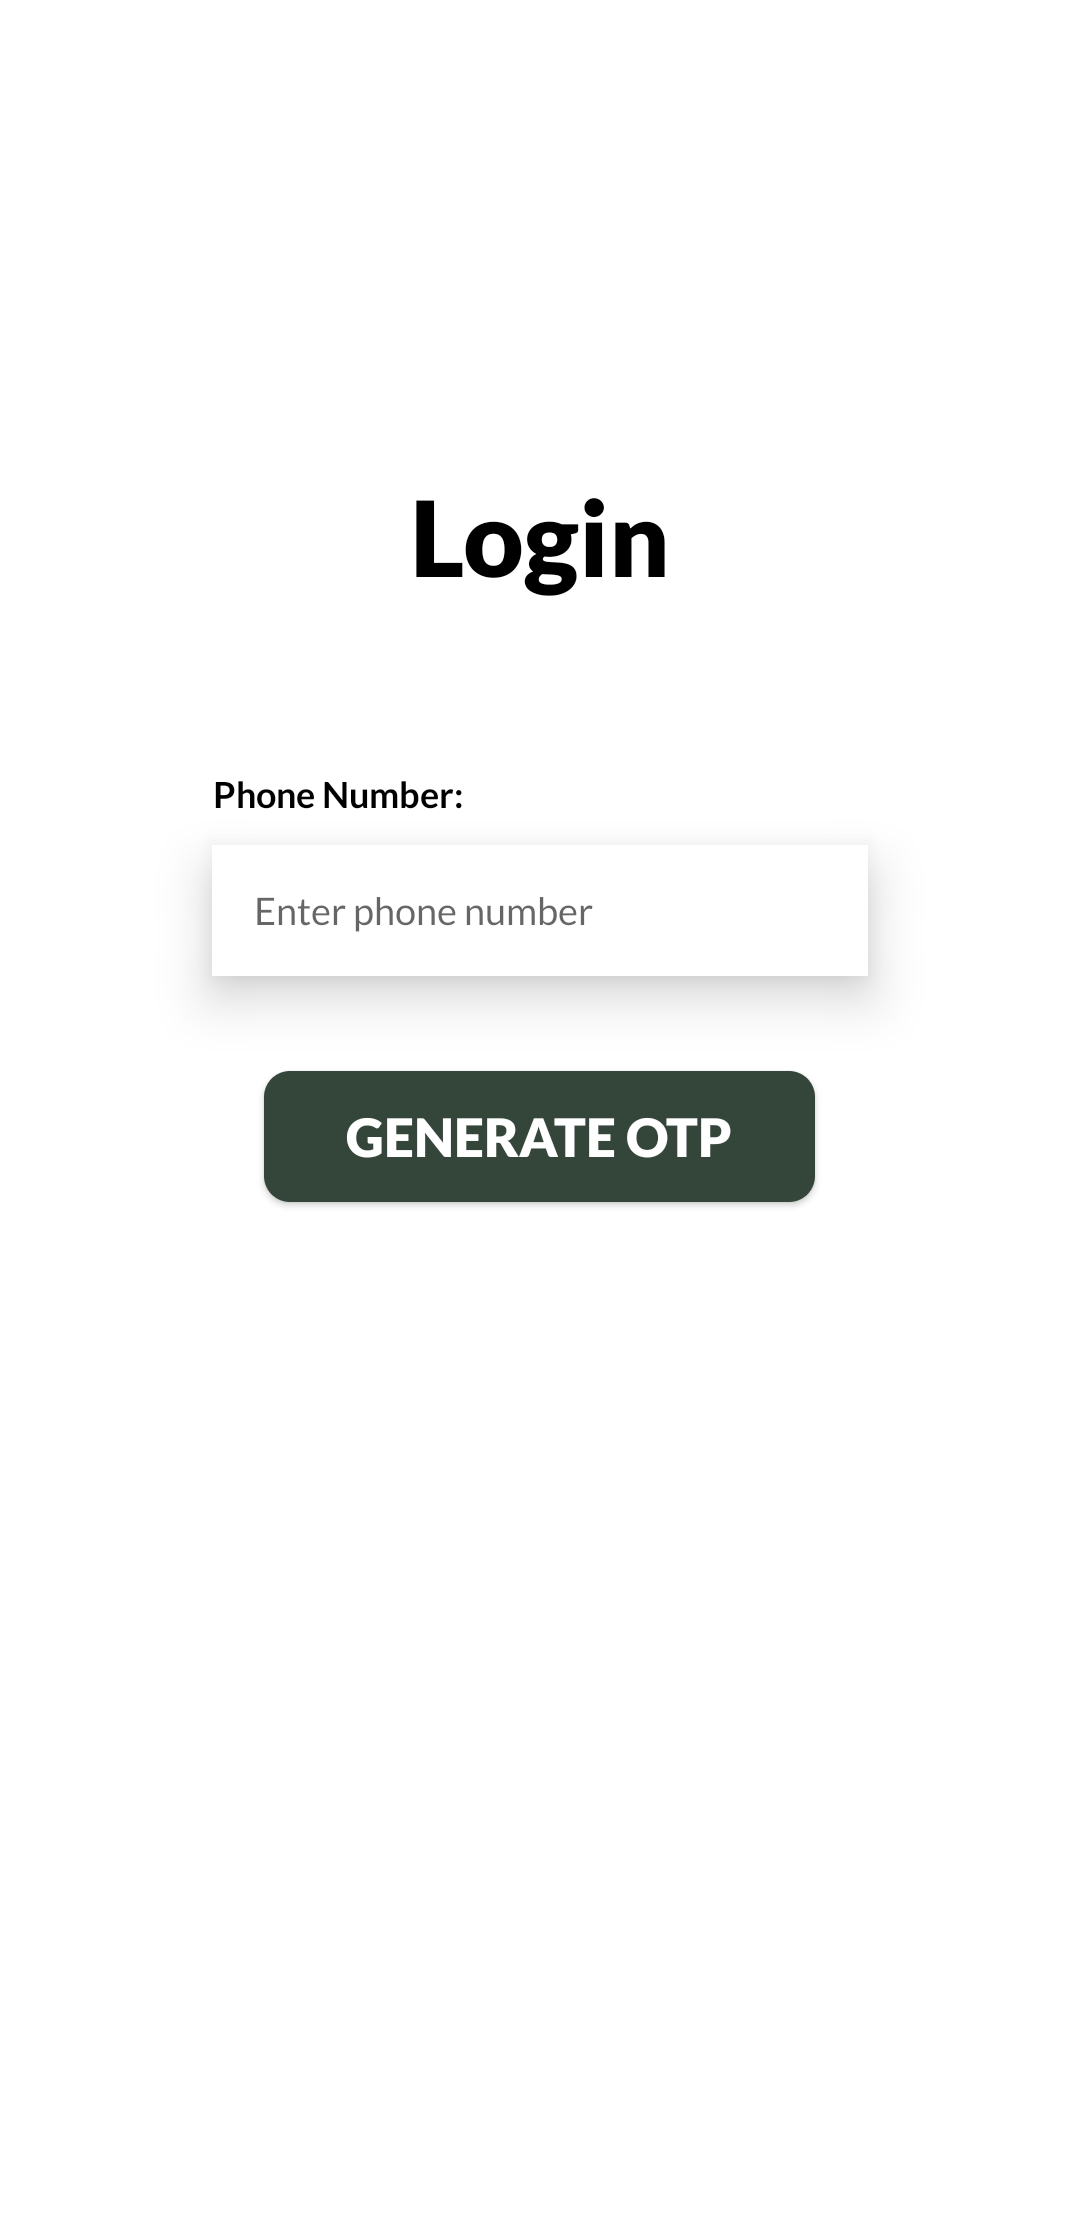
\includegraphics[width=0.5\linewidth,frame]{login.jpg}}
  \caption{Login Page}
\end{figure}

\begin{figure}[htbp]
  \centering
  \fbox{
\includegraphics[width=0.5\linewidth]{otp.jpg}}
  \caption{Authentication Page}
\end{figure}

\begin{figure}[htbp]
  \centering
  \fbox{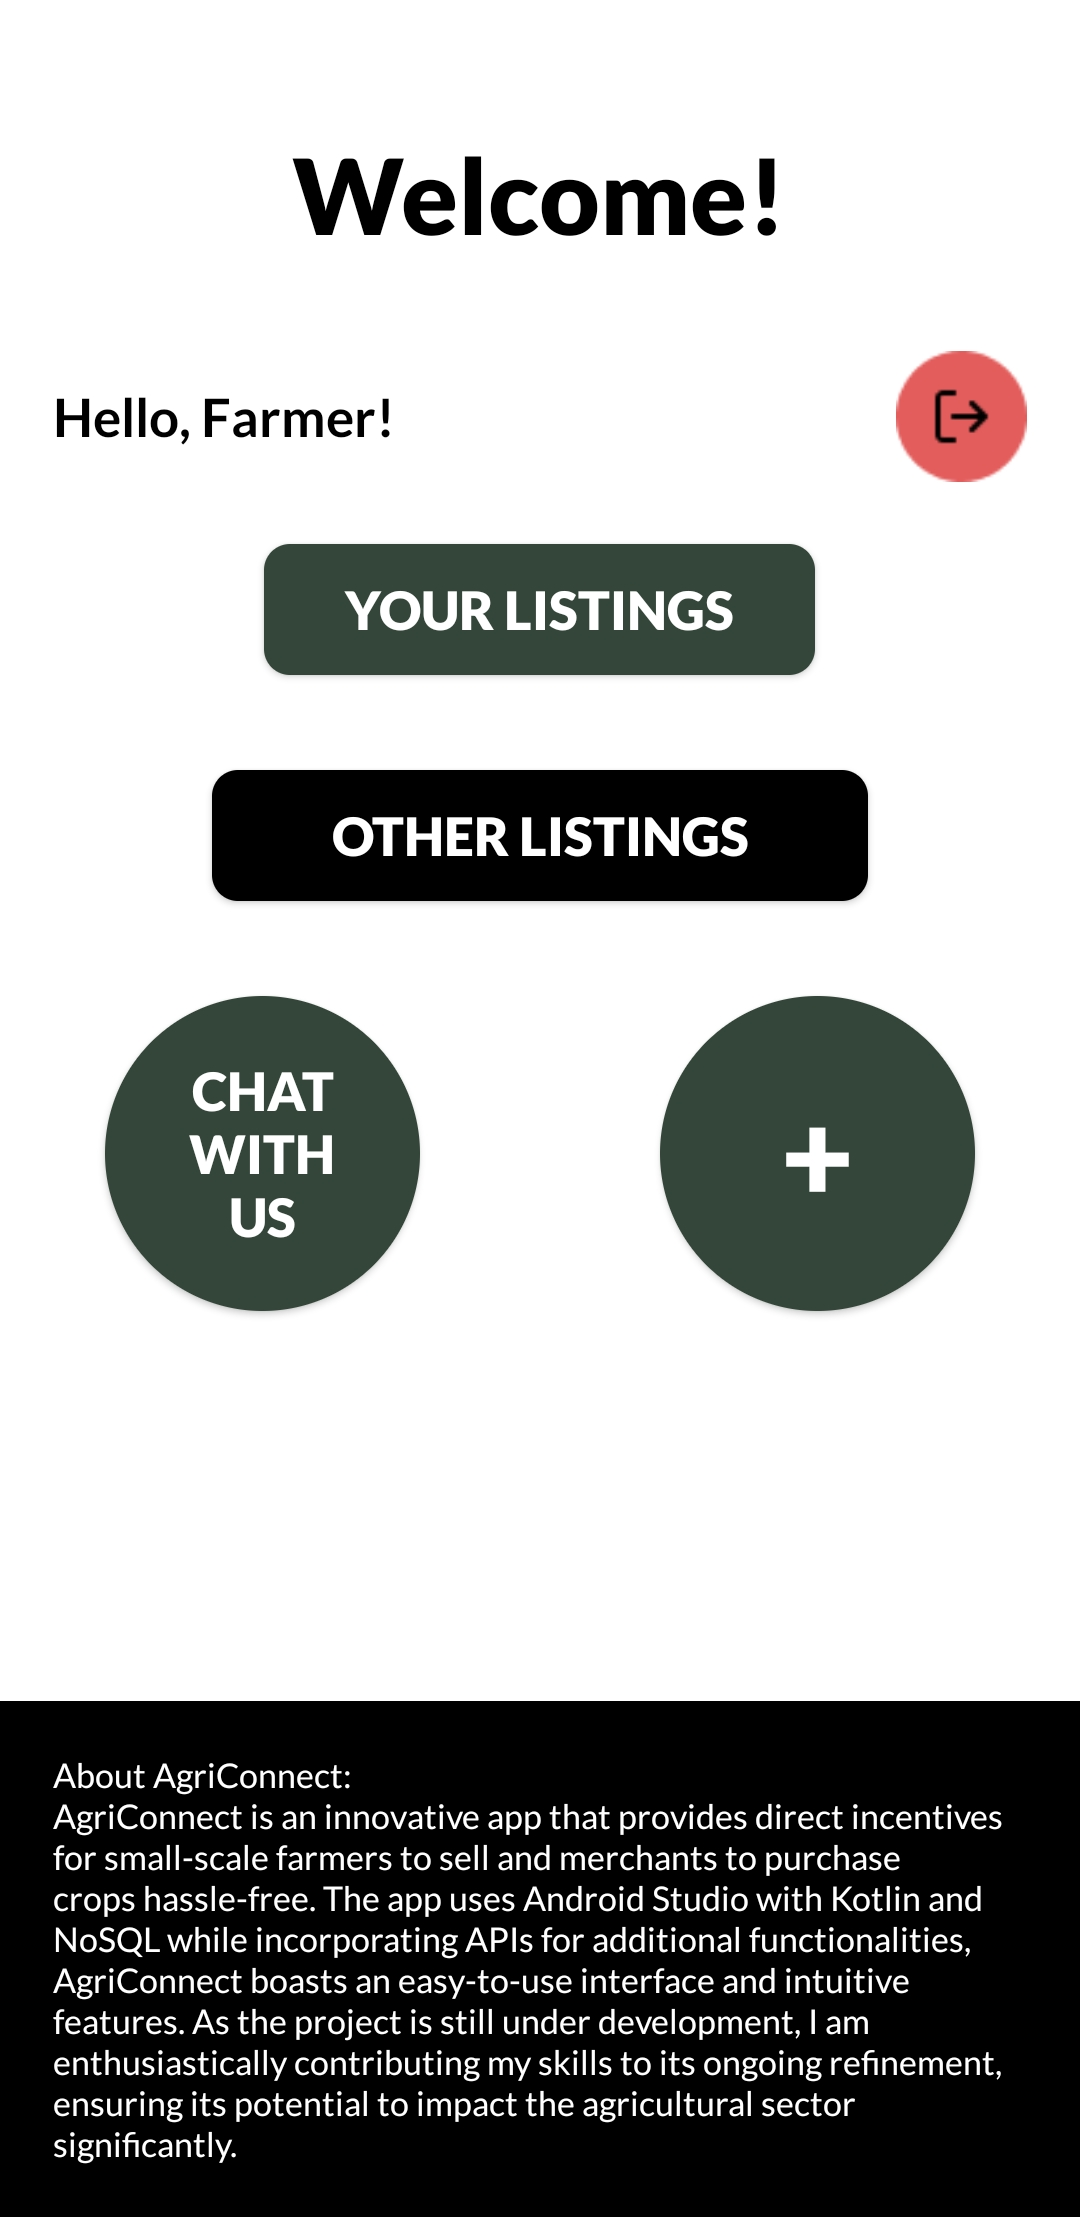
\includegraphics[width=0.5\linewidth]{home.jpg}}
  \caption{Home Page}
\end{figure}

\begin{figure}[htbp]
  \centering
  \fbox{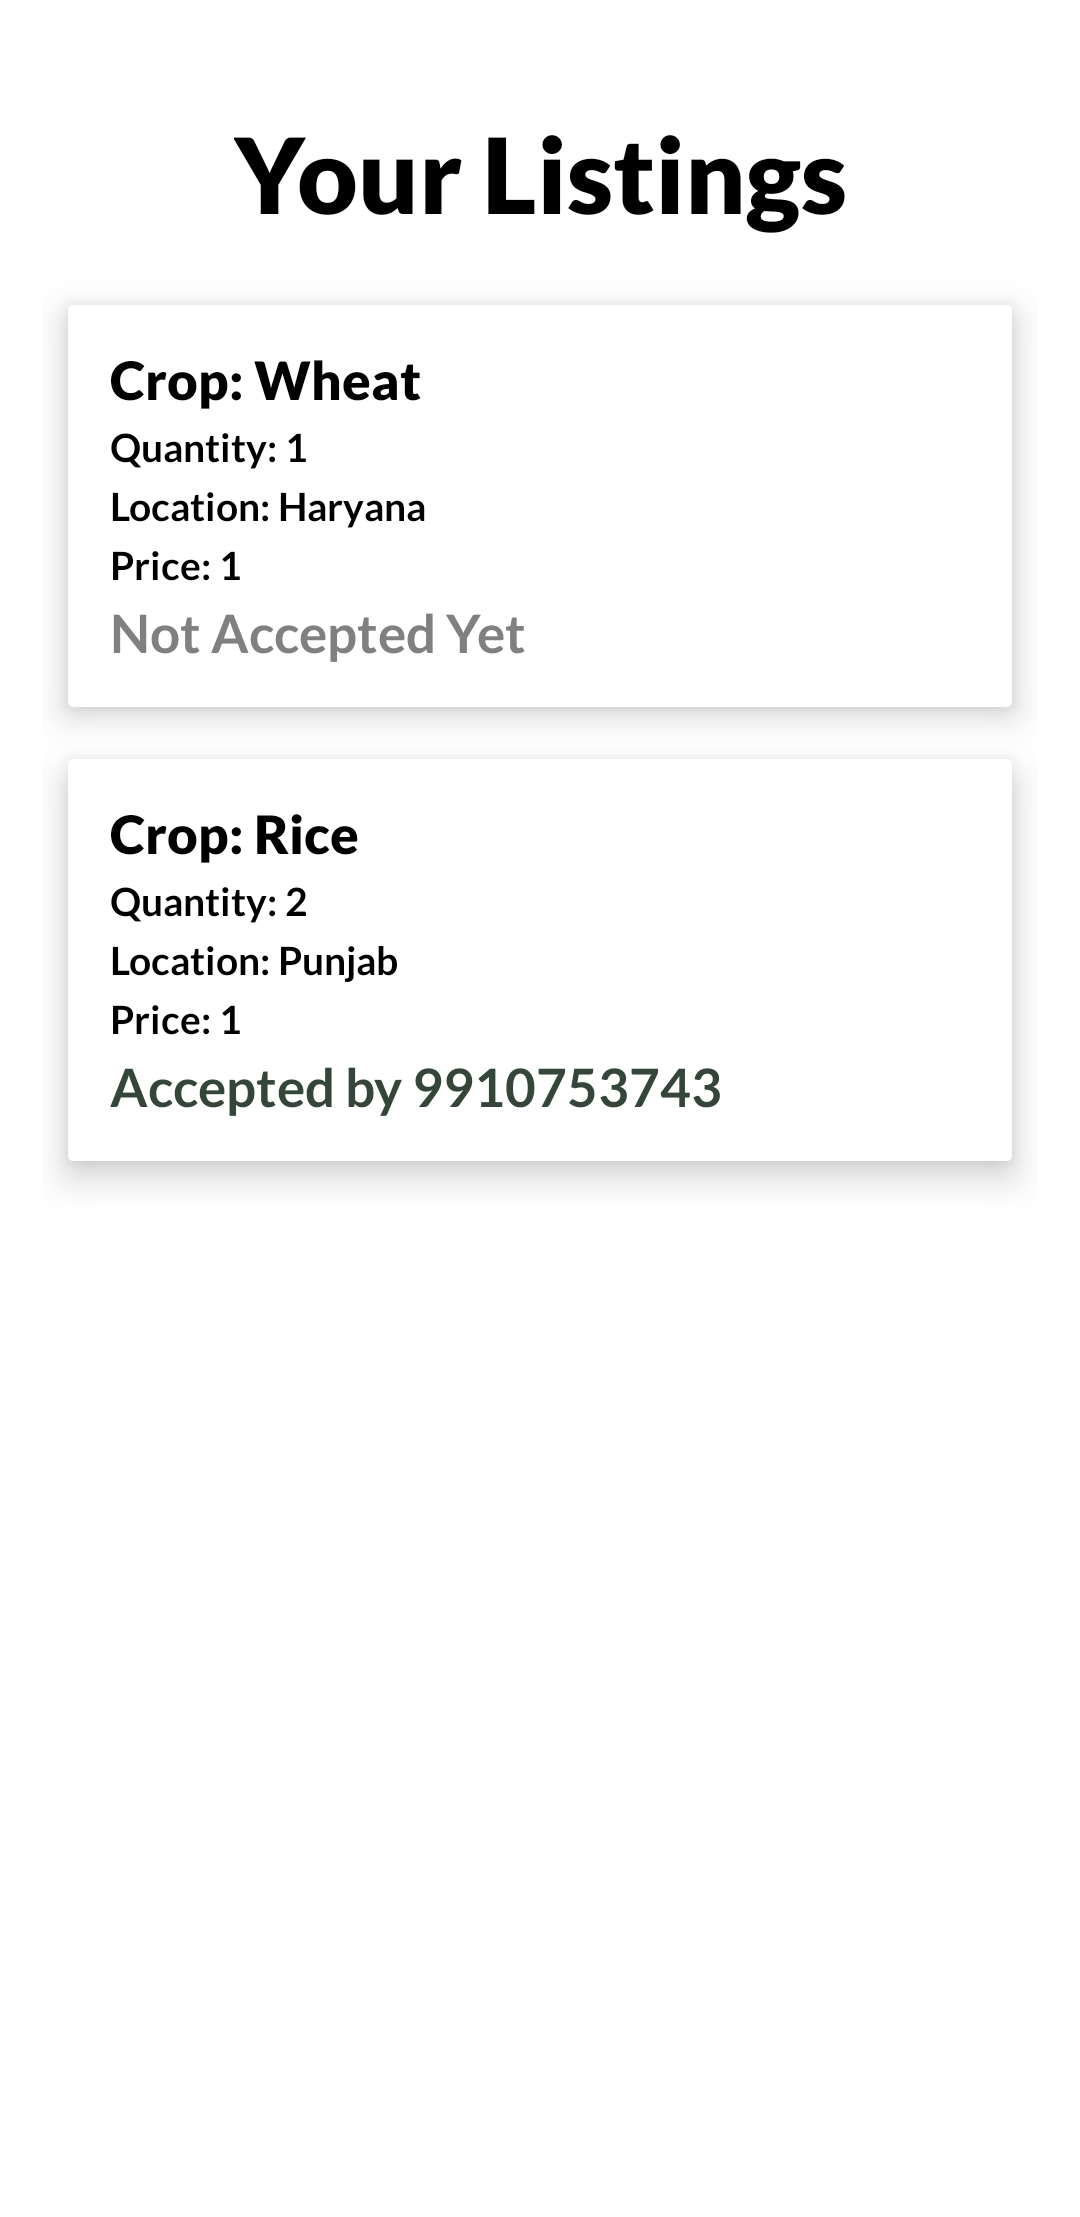
\includegraphics[width=0.5\linewidth]{yourlistingfarmer.jpg}}
  \caption{Farmer Listings for Farmer Page}
\end{figure}

\begin{figure}[htbp]
  \centering
  \fbox{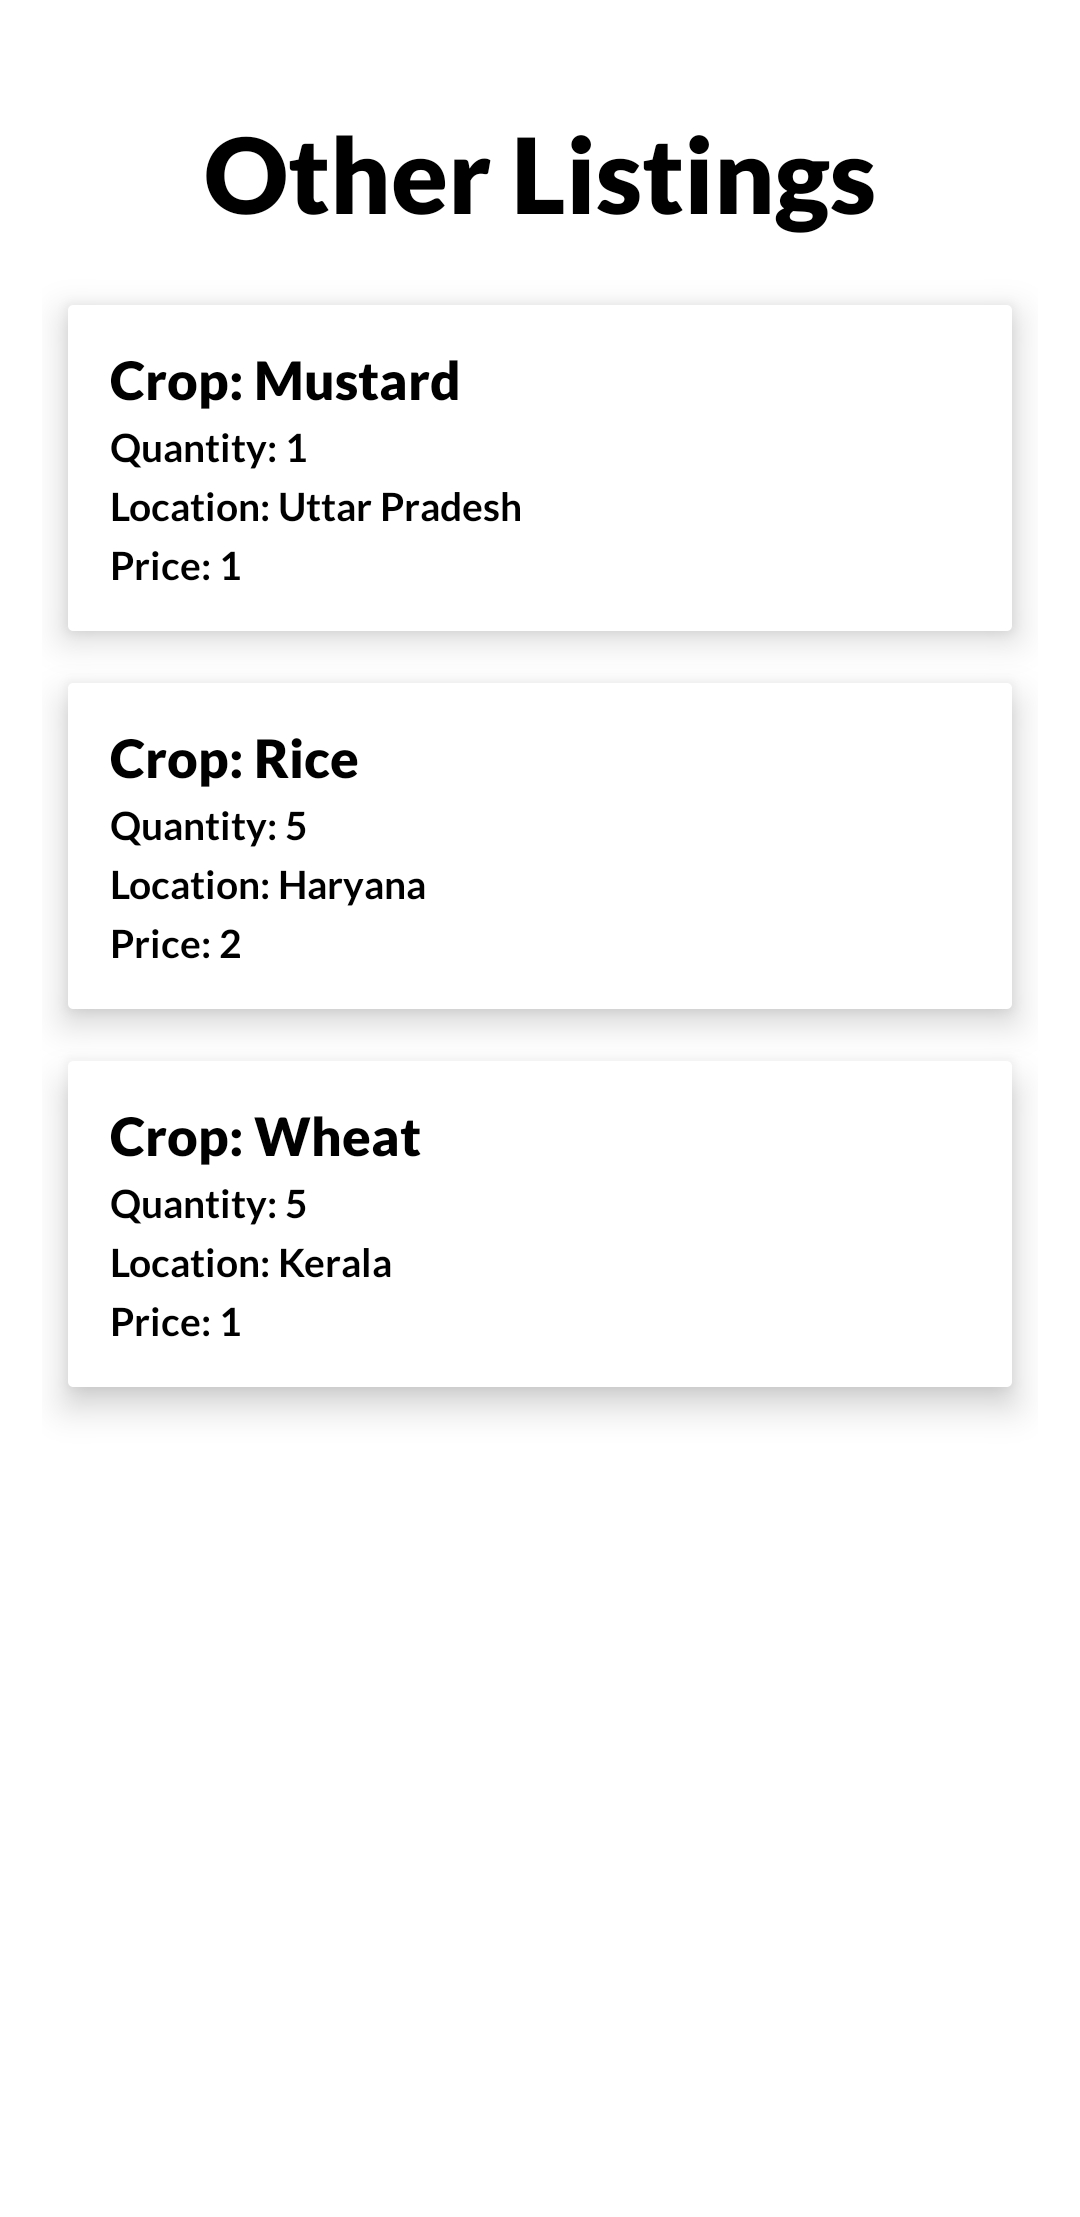
\includegraphics[width=0.5\linewidth]{otherlistingfarmer.jpg}}
  \caption{Merchant Listings for Farmer Page}
\end{figure}

\begin{figure}[htbp]
  \centering
  \fbox{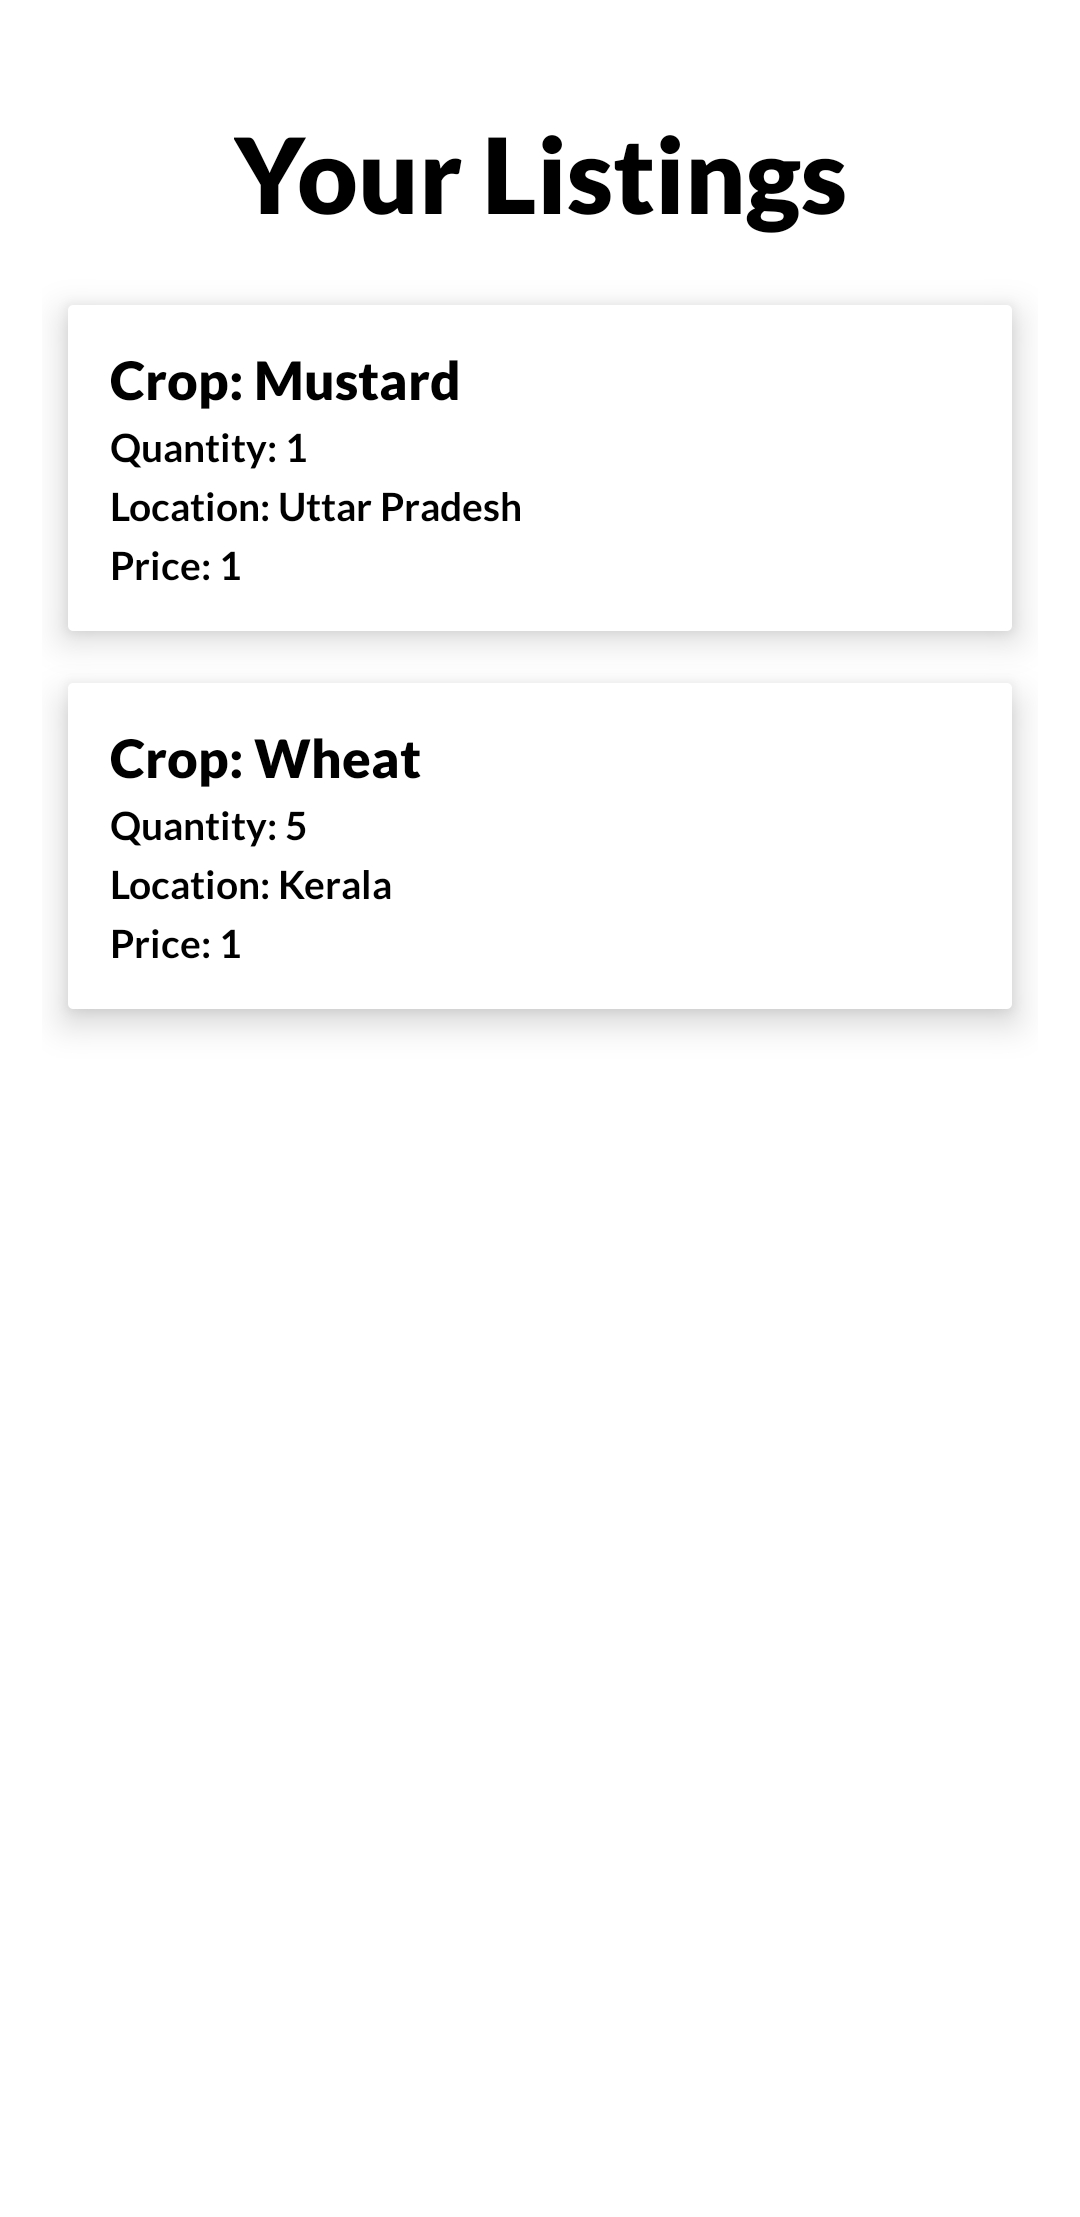
\includegraphics[width=0.5\linewidth]{yourlistingmerchant.jpg}}
  \caption{Farmer Listings for Merchant Page}
\end{figure}

\begin{figure}[htbp]
  \centering
  \fbox{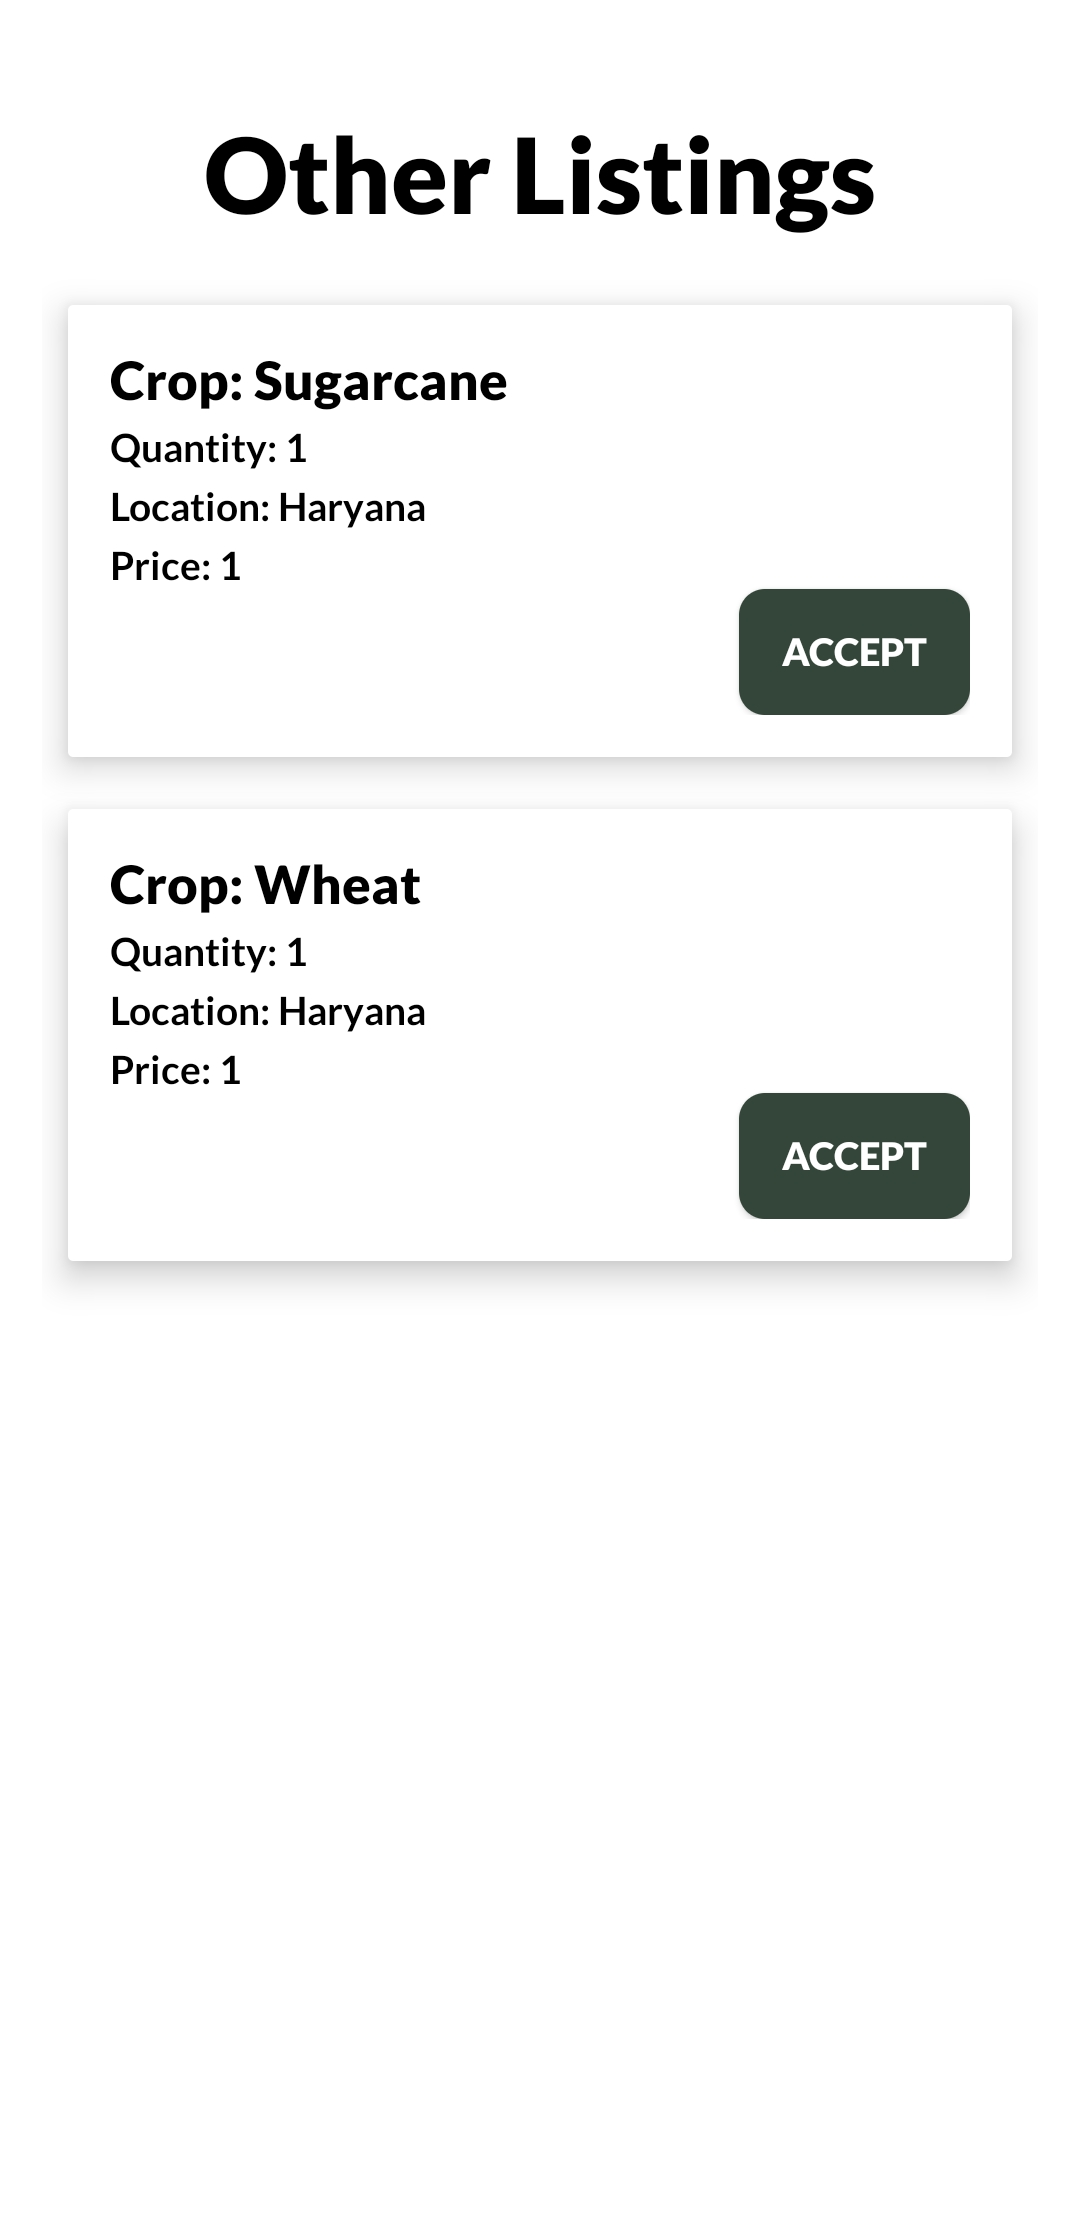
\includegraphics[width=0.5\linewidth]{otherlistingmerchant.jpg}}
  \caption{Merchant Listings for Merchant Page}
\end{figure}

\begin{figure}[htbp]
  \centering
  \fbox{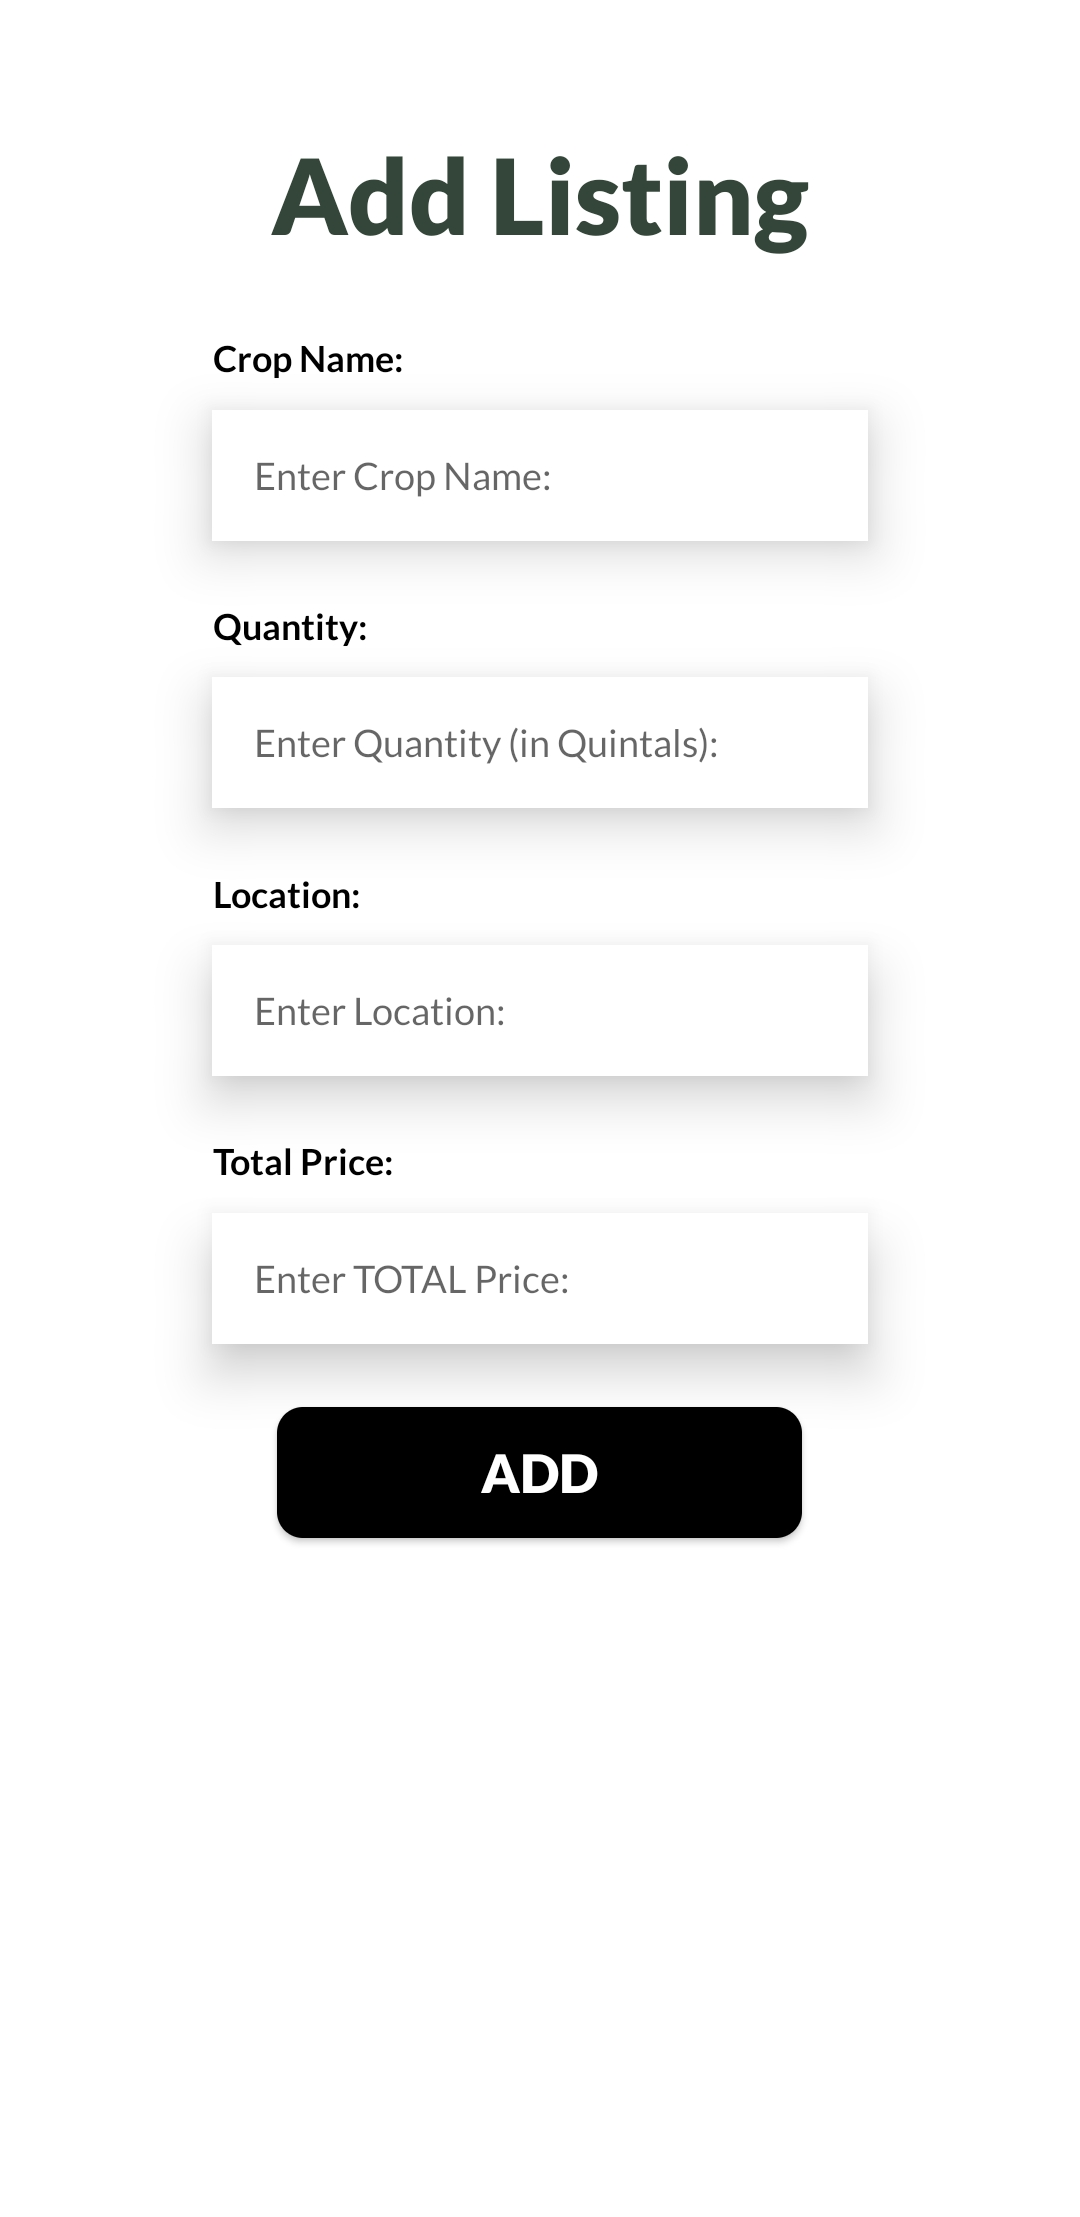
\includegraphics[width=0.5\linewidth]{addlisting.jpg}}
  \caption{Add Listings Page}
\end{figure}

\begin{figure}[htbp]
  \centering
  \fbox{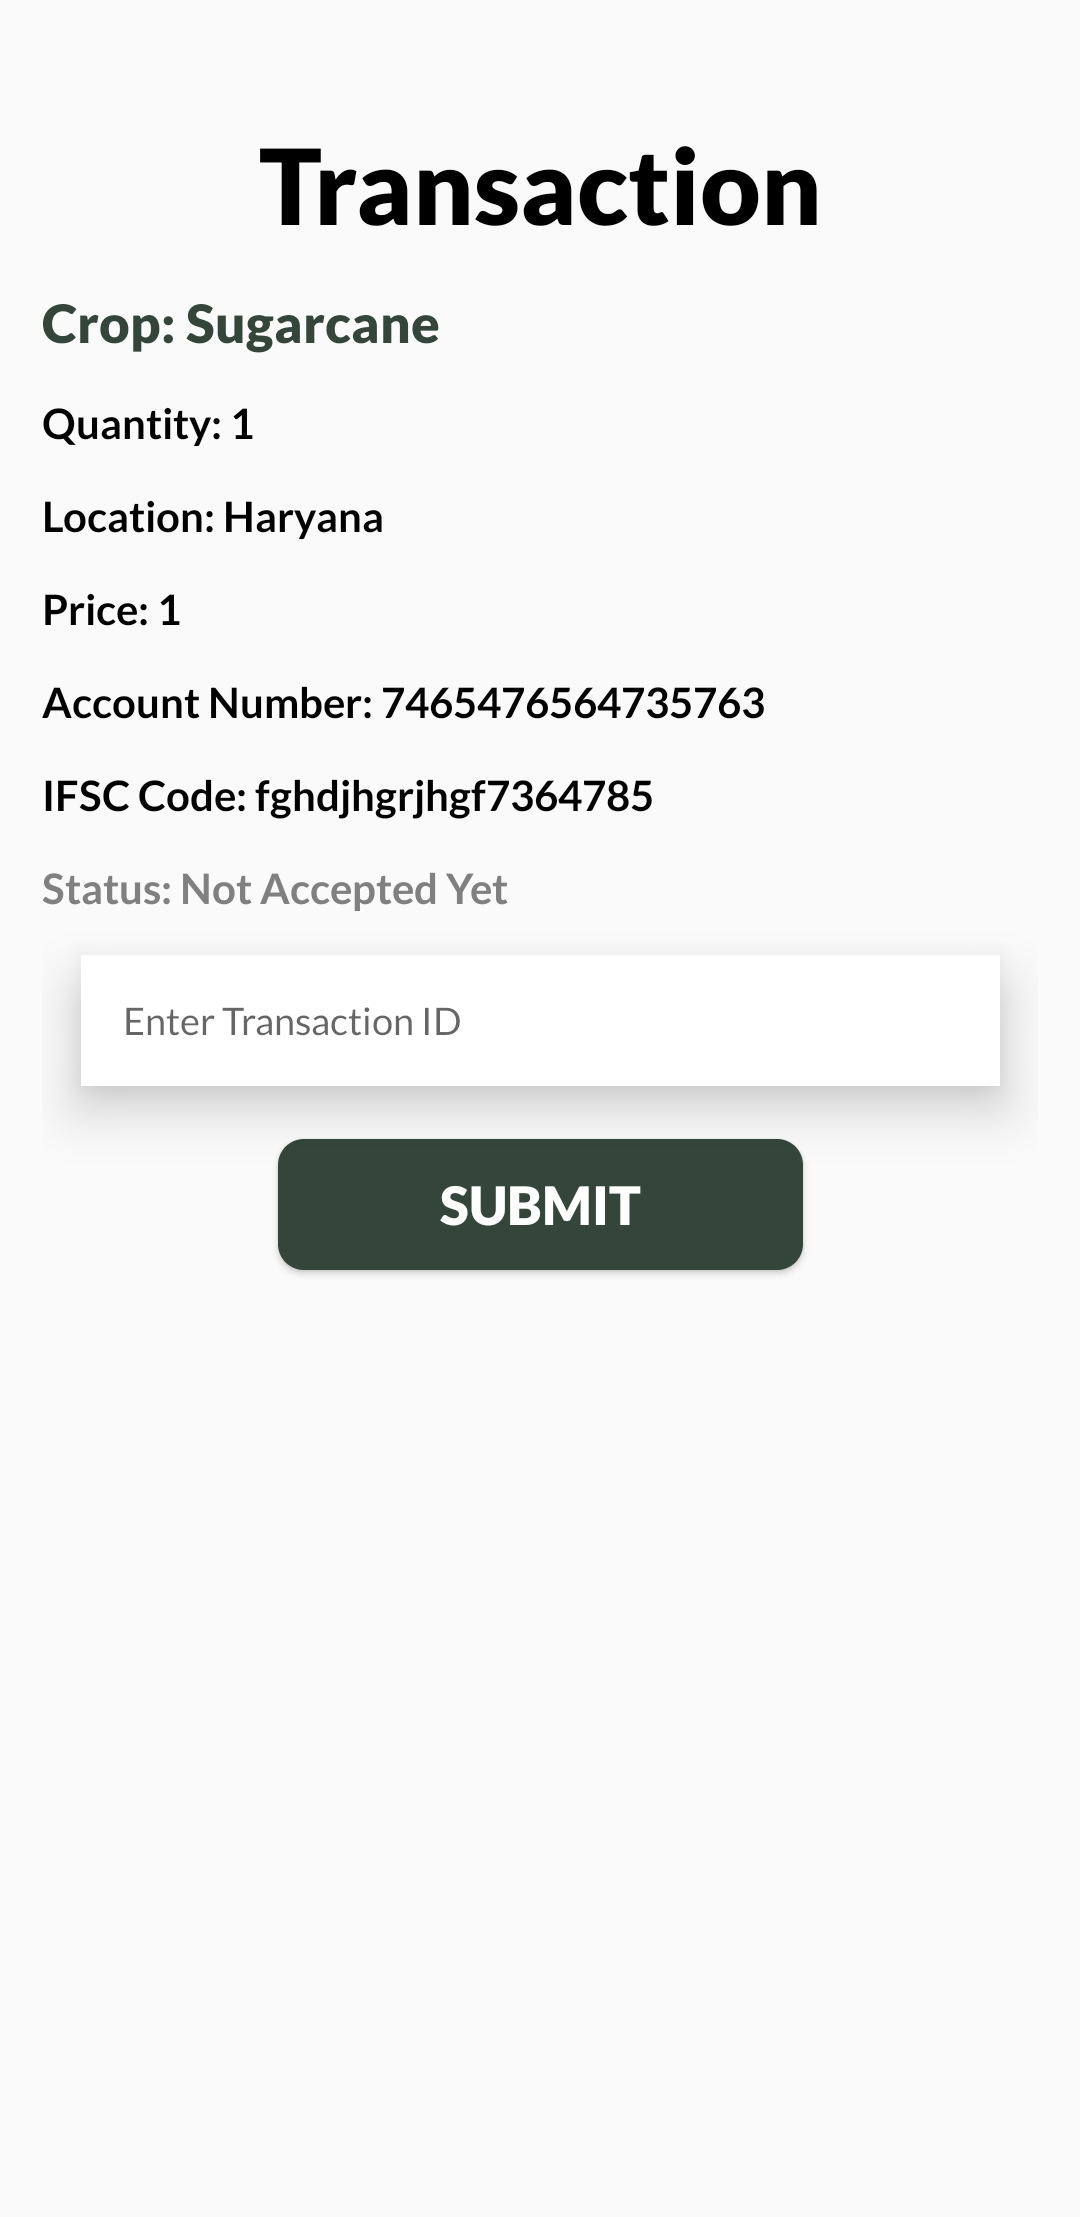
\includegraphics[width=0.5\linewidth]{transaction.jpg}}
  \caption{Transaction Page}
\end{figure}
\FloatBarrier
\section{Conclusion}
AgriConnect represents a significant step forward in leveraging technology to empower small-scale farmers and merchants. By addressing critical pain points in the agricultural supply chain with a user-friendly, accessible app, it paves the way for a more equitable and efficient marketplace. This project not only showcases the potential of mobile technology to transform traditional industries but also underscores the importance of designing with the end-user in mind, ensuring technology serves as a tool for empowerment and economic advancement. In future, we plan to add a proper transaction API to handle transactions, 

\bibliographystyle{IEEEtran} 
\bibliography{IEEEexample}

\begin{enumerate}
  \renewcommand{\theenumi}{[\arabic{enumi}]}
  \item M. Bhende, M. S. Avatade, S. Patil, P. Mishra, P. Prasad and S. She-walkar, ”Digital Market: E-Commerce Application For Farmers,” 2018 Fourth International Conference on Computing Communication Control and Automation (ICCUBEA), Pune, India, 2018, pp. 1-7.
  \item S. Rahayu, L. Fitriani, R. Kurniawati, and Y. Bustomi, ”E-commerce based on the Marketplace in efforts to sell agricultural products using Xtreme programming approach,” in Journal of Physics: Conference Series, vol. 1402, no. 6, IOP Publishing Ltd, 2019, paper 066108.
  \item N. Imesha et al., ”Building a Digital Bridge Between Sri Lankan Farmers and Retailers: Conceptual Mobile Application Prototype,” 2023 IEEE 17th International Conference on Industrial and Information Systems (ICIIS), Peradeniya, Sri Lanka, 2023, pp. 115-120.
  \item R. Deshmukh, G. Dhabadge, K. Kuvlekar, N. Kumbhar, and R. Igave, ”E-Business in Agriculture for Effective Communication between Merchants and Farmers,” in International Journal of Computer Applications, vol. 179, pp. 1-4, 2018.
  \item A. Raj, V. Kumar, and P. Singh, ”Development of a Farmer-Centric Mobile Application for Agro-Advisory Services,” International Journal of Agricultural and Biological Engineering, vol. 13, no. 3, pp. 128–134, 2020.
  \item A. Singh, P. Sharma, and R. Singh, ”A Review on Mobile Applications for Farmer Centric Agriculture,” International Journal of Advanced Research in Computer Science, vol. 10, no. 5, pp. 75–79, 2019.
  \item S. Ahmad, A. S. Abdullah, and S. Shaikh, ”Mobile Applications for Farmers: A Comprehensive Review and Future Direction,” International Journal of Advanced Computer Science and Applications, vol. 9, no. 7, pp. 140–145, 2018.
  \item Y. Zhai, H. Zhang, and X. Chen, ”A Survey on Mobile Agricultural Applications: A User Perspective,” International Journal of Agricultural and Biological Engineering, vol. 10, no. 5, pp. 153–160, 2017.
  \item A. P. Muhammed, C. J. Shon, P. S. Shemeera, P. M. Arya, and K. V. Viswam, ”AGRIO APP: An Advanced Android Application For Farmers.”
  \item K. Gurjar et al., ”Development of a Mobile Application for Connecting Farmers with Traders and a Price Prediction Model using Machine Learning,” International Research Journal of Engineering and Technology (IRJET), vol. 10, no. 10, pp. 663, Oct. 2023.
  \item A. Bhandari et al., ”ANDROID APPLICATION FOR FARMERS TO SELL THEIR PRODUCEATBETTERRATES,” International Research Journal of Modernization in Engineering Technology and Science, vol. 03, no. 01, Jan. 2021, pp. 393.
  \item M. Dane et al., ”E-Farming Bazaar,” IJSRD- International Journal for Scientific Research Development, vol. 6, no. 03, 2018, pp. 447.
\end{enumerate}

\end{document}


